\documentclass[11pt]{article}

\usepackage[margin=1in]{geometry}
\usepackage{amsmath}
\usepackage{booktabs}
\usepackage{array}
\usepackage{enumitem}
\usepackage{float}
\usepackage{graphicx}
\usepackage{hyperref}
\usepackage{xcolor}
\usepackage{tikz}
\usetikzlibrary{arrows.meta, positioning, shapes.geometric}

\hypersetup{
  colorlinks=true,
  linkcolor=blue!60!black,
  citecolor=blue!60!black,
  urlcolor=blue!60!black
}

\setlist[itemize]{leftmargin=1.3em}
\setlist[enumerate]{leftmargin=1.5em}
\renewcommand{\arraystretch}{1.15}

\title{\textbf{LLM-Augmented High-Level Route Planning for Autonomous UAV Navigation}}
\author{
Prachit Gupta\\
}
\date{\today}

\begin{document}
\maketitle

\begin{abstract}
This report presents an LLM-augmented high-level route-planning framework for autonomous UAV navigation on the ModalAI Starling 2 platform. The system uses perception-derived obstacle descriptions, structured prompting, sparse waypoint generation, waypoint interpolation, verification-based safety filtering, and PX4 trajectory execution. The LLM is not used as a real-time motion planner. Instead, it acts as a semantic mission planner that converts natural language objectives and scene context into sparse NED-frame waypoints. Classical refinement and verification modules then enforce geometric and kinematic constraints before the verified trajectory is latched by the low-level controller. The implementation is available in the project repository:
\url{https://github.com/prachitgupta/starling_testing_ws}.
\end{abstract}

\section{Introduction and Motivation}

Autonomous navigation for unmanned aerial vehicles (UAVs) has traditionally relied on classical path-planning algorithms such as A*, RRT, RRT*, optimization-based planners, and reinforcement-learning policies. These approaches provide strong geometric reasoning, collision checks, and mathematically grounded trajectory generation. However, such methods are limited in semantic awareness, contextual understanding, and human-interpretable decision making. Traditional planners are largely blind to natural language instructions, environmental semantics, and human intent. They usually require explicitly defined waypoint coordinates, handcrafted cost functions, or large amounts of environment-specific training data.

Recent advances in large language models (LLMs) and vision-language models (VLMs) have demonstrated strong capabilities in semantic reasoning, contextual awareness, human-aligned decision making, and generalization across domains. Unlike conventional path-planning methods, LLMs are trained on large human-generated datasets and therefore encode useful high-level reasoning patterns. This creates an opportunity to bridge the semantic gap between human intent and robotic execution.

Instead of requiring expert UAV operators to provide precise waypoint coordinates or manually designed mission specifications, natural language instructions can be translated into actionable navigation objectives. For example, instead of specifying an exact spatial coordinate, a user may provide an instruction such as:

\begin{quote}
``Navigate to the chair near the whiteboard while avoiding nearby obstacles.''
\end{quote}

An LLM can interpret the semantic structure of the instruction, infer contextual relationships between objects, and generate sparse waypoint sequences corresponding to the intended high-level route. This significantly reduces dependency on expert operators and enables more intuitive human-robot interaction.

This motivation is especially relevant in modern human-centric environments where robots are expected to coexist and collaborate with humans. Earlier robotics applications often focused on environments inaccessible to humans. Modern autonomous systems, including self-driving vehicles, collaborative drones, and assistive robots, increasingly operate in shared environments. Consequently, high-level mission planning must align closely with human intent and contextual reasoning rather than relying only on geometric optimization.

The central hypothesis explored in this work is that LLM-generated sparse waypoint trajectories, when augmented with refinement and verification tools, can serve as effective high-level route plans for UAV navigation. Rather than relying on LLMs for low-level control or real-time trajectory optimization, the framework leverages their strengths in semantic reasoning, contextual interpretation, and generalization while delegating geometric feasibility and collision checking to traditional modules.

\section{Problem Statement}

The objective of this project is to investigate whether large language models can be reliably used for high-level UAV route planning when augmented with appropriate perception, refinement, and verification pipelines.

The project explores the following research questions:

\begin{enumerate}
  \item Can LLMs generate semantically meaningful sparse waypoint trajectories from natural language instructions and environmental context?
  \item Can refinement and verification pipelines compensate for the poor spatial interpretability and numerical inaccuracies of LLM-generated outputs?
  \item Can LLM-generated high-level plans be deployed successfully on real UAV hardware platforms?
  \item To what extent can LLM-based planning provide human-aligned and semantically aware navigation behavior compared to traditional planning approaches?
\end{enumerate}

\section{Related Work}
More details are provided in \texttt{short\_survey.pdf}.

Classical path-planning methods such as A*, RRT, and optimization-based planners remain highly effective in environments where geometric structure and obstacle maps are explicitly known. These methods can provide mathematical guarantees regarding completeness, collision avoidance, and optimality. However, they fundamentally lack semantic awareness and contextual understanding. They do not directly reason about movable obstacles, human intent, or contextual object relationships.

Learning-based approaches such as reinforcement learning and imitation learning have also demonstrated strong performance in UAV navigation tasks. However, these methods generally require large amounts of environment-specific training data and often fail to generalize reliably to unseen environments.

Recent research involving foundation models, LLMs, and VLMs has demonstrated promising capabilities in robotics, navigation, reasoning, and multimodal perception. Prior work such as FM-Planner has explored the use of LLMs and VLMs for drone navigation by generating sparse waypoints using textual prompts and visual encoders. This project follows a similar conceptual direction while focusing specifically on hardware deployability, high-level semantic route planning, verification-augmented planning, and real-world UAV experimentation.

Unlike approaches that attempt to use LLMs directly for real-time motion planning, this work explicitly separates semantic route planning, geometric refinement, low-level trajectory tracking, and safety verification.

\section{Codebase and Implementation Overview}

The implementation is organized in the ROS 2 package \texttt{llm\_vision\_planner}. The main pipeline is launched through:

\begin{center}
\url{https://github.com/prachitgupta/starling_testing_ws/blob/main/src/llm_vision_planner/launch/full_plot.launch.py}
\end{center}

The launch file starts the following nodes:

\begin{itemize}
  \item \texttt{semantic\_obstacle\_perception}: combines point-cloud clustering with semantic labels from \texttt{/tflite\_data}.
  \item \texttt{obstacle\_perception}: fallback geometric point-cloud obstacle detector.
  \item \texttt{prompt\_generator}: converts pose, goal, workspace, and obstacles into a structured natural-language prompt.
  \item \texttt{llm\_planner}: calls the OpenAI model through Instructor and validates the structured sparse waypoint response.
  \item \texttt{path\_refinement}: interpolates and sanitizes the sparse plan.
  \item \texttt{path\_verifier}: computes safety, kinematic, workspace, and goal metrics.
  \item \texttt{planner\_visualizer}: plots sparse, refined, and verified trajectories.
\end{itemize}

The key implementation files are:

\begin{itemize}
  \item Prompt generation: \url{https://github.com/prachitgupta/starling_testing_ws/blob/main/src/llm_vision_planner/scripts/prompt_generator.py}
  \item LLM planner: \url{https://github.com/prachitgupta/starling_testing_ws/blob/main/src/llm_vision_planner/scripts/llm_planner.py}
  \item Refinement: \url{https://github.com/prachitgupta/starling_testing_ws/blob/main/src/llm_vision_planner/scripts/refinment.py}
  \item Verification: \url{https://github.com/prachitgupta/starling_testing_ws/blob/main/src/llm_vision_planner/scripts/verifier.py}
  \item PX4 trajectory follower: \url{https://github.com/prachitgupta/starling_testing_ws/blob/main/src/llm_vision_planner/scripts/trajectory_follower.py}
  \item Hardware test README: \url{https://github.com/prachitgupta/starling_testing_ws/blob/main/src/llm_vision_planner/HARDWARE_TESTING_README.md}
\end{itemize}

\section{Proposed Framework}

The proposed framework combines natural language reasoning, vision-based obstacle perception, sparse waypoint generation, trajectory refinement, and verification-based safety filtering. The LLM is used exclusively for high-level route planning and not for real-time control.

\begin{figure}[H]
\centering
\resizebox{\textwidth}{!}{
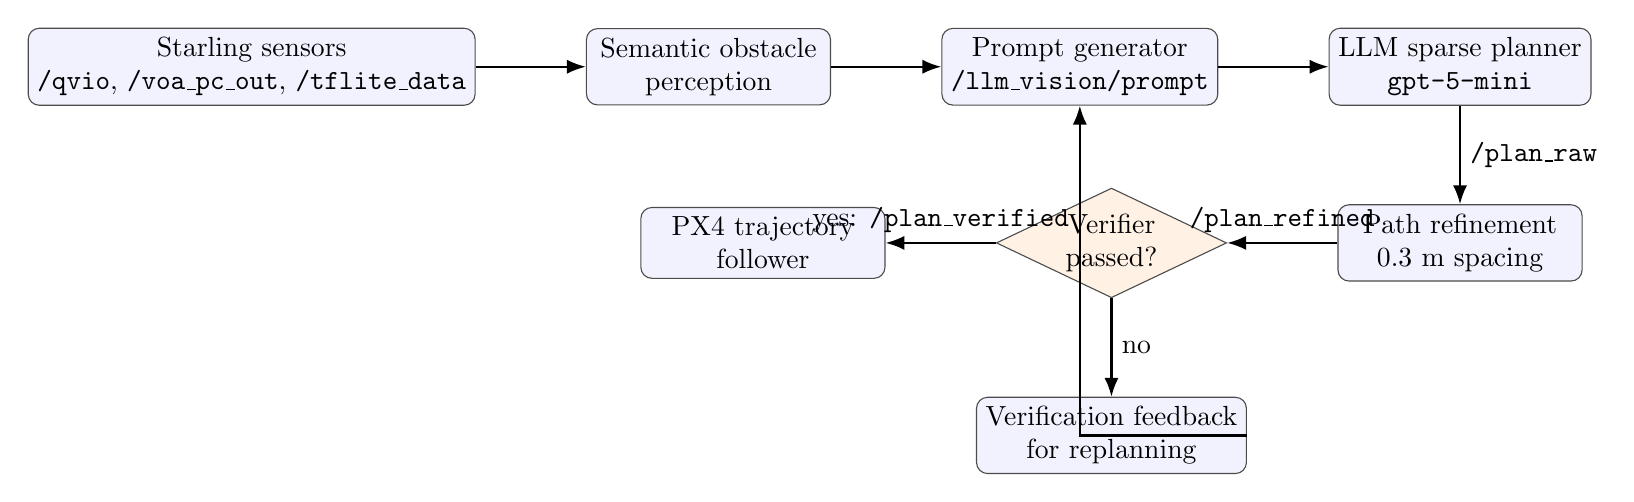
\begin{tikzpicture}[
  node distance=1.25cm and 1.4cm,
  block/.style={rectangle, rounded corners, draw=black!70, fill=blue!5, minimum width=3.1cm, minimum height=0.9cm, align=center},
  check/.style={diamond, aspect=2.1, draw=black!70, fill=orange!10, align=center, inner sep=1pt},
  arrow/.style={-{Latex[length=2.4mm]}, thick}
]
\node[block] (sensors) {Starling sensors\\\texttt{/qvio}, \texttt{/voa\_pc\_out}, \texttt{/tflite\_data}};
\node[block, right=of sensors] (perception) {Semantic obstacle\\perception};
\node[block, right=of perception] (prompt) {Prompt generator\\\texttt{/llm\_vision/prompt}};
\node[block, right=of prompt] (llm) {LLM sparse planner\\\texttt{gpt-5-mini}};
\node[block, below=of llm] (refine) {Path refinement\\0.3 m spacing};
\node[check, left=of refine] (verify) {Verifier\\passed?};
\node[block, left=of verify] (follower) {PX4 trajectory\\follower};
\node[block, below=of verify] (feedback) {Verification feedback\\for replanning};

\draw[arrow] (sensors) -- (perception);
\draw[arrow] (perception) -- (prompt);
\draw[arrow] (prompt) -- (llm);
\draw[arrow] (llm) -- node[right]{\texttt{/plan\_raw}} (refine);
\draw[arrow] (refine) -- node[above]{\texttt{/plan\_refined}} (verify);
\draw[arrow] (verify) -- node[above]{yes: \texttt{/plan\_verified}} (follower);
\draw[arrow] (verify) -- node[right]{no} (feedback);
\draw[arrow] (feedback.east) -| (prompt.south);
\end{tikzpicture}}
\caption{LLM-augmented UAV planning pipeline implemented in \texttt{llm\_vision\_planner}.}
\label{fig:pipeline}
\end{figure}

The pipeline operates as follows:

\begin{enumerate}
  \item Natural language mission instructions are combined with onboard pose, workspace limits, goal position, and obstacle information.
  \item The perception node produces structured obstacle descriptions containing labels, centroids, bounding boxes, sizes, bearings, and distances.
  \item The prompt generator publishes a single structured prompt on \texttt{/llm\_vision/prompt}.
  \item The LLM returns a sparse sequence of NED-frame waypoints through a Pydantic response model.
  \item The refinement node interpolates intermediate waypoints every \texttt{0.3 m}, clamps points to the workspace, and nudges non-goal points away from obstacle boxes.
  \item The verifier computes safety and feasibility metrics.
  \item If verification fails, the result can be fed back into the prompt-generation loop for another attempt.
  \item Once a trajectory passes verification, it is latched by the PX4 trajectory follower and executed.
  \item During execution, the LLM is no longer queried unless replanning is required.
\end{enumerate}

\section{Vision-Based Perception Pipeline}

Initial experiments attempted to use raw depth-camera point cloud information generated from the Starling platform's onboard sensors. Real-world indoor environments produced noisy and unreliable point-cloud maps due to occlusions, clutter, lighting disturbances, shadows, reflective surfaces, and sensor noise. The perception pipeline frequently mistook noise and shadows for obstacles while simultaneously failing to detect valid obstacles in some scenarios. Extracting reliable obstacle representations from raw depth feeds required filtering, clustering, and segmentation pipelines, increasing implementation complexity.

The implemented semantic perception node uses \texttt{/voa\_pc\_out} point clouds, \texttt{/qvio} pose estimates, and \texttt{/tflite\_data} semantic detections. The point cloud is filtered by range and clustered using DBSCAN. Each cluster is converted into a structured obstacle object:

\begin{itemize}
  \item centroid,
  \item minimum and maximum 3D corners,
  \item size,
  \item distance from the UAV,
  \item bearing angle,
  \item semantic label,
  \item point count.
\end{itemize}

The configured semantic perception parameters are listed in Table~\ref{tab:perception-params}. The implementation also supports a normal point-cloud-only mode, but the semantic mode is used for the main hardware pipeline.

\begin{table}[H]
\centering
\caption{Configured perception parameters.}
\label{tab:perception-params}
\begin{tabular}{lll}
\toprule
Parameter & Value & Meaning \\
\midrule
\texttt{point\_cloud\_topic} & \texttt{/voa\_pc\_out} & Depth/VOA point cloud input \\
\texttt{pose\_topic} & \texttt{/qvio} & Visual-inertial odometry input \\
\texttt{detection\_topic} & \texttt{/tflite\_data} & Semantic object detection input \\
\texttt{obstacle\_topic} & \texttt{/llm\_vision/semantic\_obstacles} & Published obstacle descriptor \\
\texttt{min\_range\_m} & 0.15 & Minimum point range retained \\
\texttt{max\_range\_m} & 4.0 & Maximum point range retained \\
\texttt{dbscan\_eps} & 0.5 & DBSCAN cluster radius \\
\texttt{dbscan\_min\_samples} & 8 & Minimum samples per cluster \\
\bottomrule
\end{tabular}
\end{table}

This design trades generality for robustness. A semantic detector can only label trained classes, but the extracted obstacle information is cleaner and more meaningful for an LLM than raw point clouds. The advantage is that the planner can reason about obstacle types, such as chairs, humans, static obstacles, movable objects, or navigable gaps.

\section{Sparse Waypoint Generation Using LLMs}

The LLM planner subscribes to \texttt{/llm\_vision/prompt} and publishes sparse plans on \texttt{/llm\_vision/plan\_raw}. The configured model is \texttt{gpt-5-mini}. The response format is enforced by a Pydantic schema through the Instructor library. The schema requires:

\begin{itemize}
  \item a short reasoning string,
  \item a list of 2 to 8 waypoints,
  \item each waypoint containing floating-point \texttt{x}, \texttt{y}, and \texttt{z} values.
\end{itemize}

The LLM output is rejected before publication if any waypoint violates the fixed altitude constraint or if the final waypoint does not match the goal within \texttt{0.05 m}. The sparse representation is intentional because LLMs are better at high-level route structure than dense numerical prediction. Dense trajectory generation is delegated to the refinement stage.

\begin{table}[H]
\centering
\caption{Example LLM sparse prediction before refinement.}
\label{tab:llm-example}
\begin{tabular}{ccccc}
\toprule
Waypoint & x (m) & y (m) & z (m) & Planner role \\
\midrule
1 & 0.10 & 0.05 & -0.45 & Start/hold vicinity \\
2 & 0.90 & 0.90 & -0.45 & Move around first obstacle \\
3 & 1.85 & 1.10 & -0.45 & Pass through open corridor \\
4 & 2.55 & 0.45 & -0.45 & Turn toward goal \\
5 & 3.00 & 0.00 & -0.45 & Goal \\
\bottomrule
\end{tabular}
\end{table}

\section{Trajectory Refinement}

The refinement module receives \texttt{/llm\_vision/plan\_raw} and publishes \texttt{/llm\_vision/plan\_refined}. Its job is to convert sparse LLM waypoints into a denser, safer sequence that the low-level PX4 follower can track.

For each consecutive sparse waypoint pair, the implementation computes the planar distance:

\[
d = \sqrt{(x_{i+1}-x_i)^2 + (y_{i+1}-y_i)^2}.
\]

It then computes the number of interpolation steps:

\[
N = \max\left(1, \left\lceil \frac{d}{s} \right\rceil\right),
\]

where the configured interpolation spacing is \(s = 0.3\) m. Intermediate waypoints are generated using linear interpolation:

\[
p(t) = p_i + t(p_{i+1}-p_i), \quad t \in \left\{\frac{1}{N}, \frac{2}{N}, \ldots, 1\right\}.
\]

The configured flight altitude is held constant at \(z=-0.45\) m. Each non-goal point is sanitized by checking whether its \(x,y\) location lies inside an obstacle box expanded by the safety margin. If it does, the point is nudged out of the closest side of the expanded box by \texttt{0.02 m}. Finally, all points are clamped to the workspace bounds \([0,4]\) m in both \(x\) and \(y\). The goal endpoint is preserved during the final interpolation step so that the verified path still terminates at the commanded goal.

\begin{table}[H]
\centering
\caption{Configured refinement parameters.}
\label{tab:refinement-params}
\begin{tabular}{lll}
\toprule
Parameter & Value & Meaning \\
\midrule
\texttt{raw\_plan\_topic} & \texttt{/llm\_vision/plan\_raw} & Input sparse plan \\
\texttt{refined\_plan\_topic} & \texttt{/llm\_vision/plan\_refined} & Output refined plan \\
\texttt{interpolation\_spacing\_m} & 0.3 & Maximum nominal spacing between samples \\
\texttt{safety\_margin\_m} & 0.40 & Obstacle-box expansion for nudging \\
\texttt{nudge\_epsilon\_m} & 0.02 & Extra push outside expanded obstacle box \\
\texttt{fixed\_z} & -0.45 & Constant NED altitude used in the plan \\
\bottomrule
\end{tabular}
\end{table}

\begin{table}[H]
\centering
\caption{Example refined path segment produced from the sparse prediction in Table~\ref{tab:llm-example}.}
\label{tab:refined-example}
\begin{tabular}{ccccc}
\toprule
Index & x (m) & y (m) & z (m) & Note \\
\midrule
1 & 0.10 & 0.05 & -0.45 & Sparse point retained \\
2 & 0.30 & 0.26 & -0.45 & Interpolated \\
3 & 0.50 & 0.47 & -0.45 & Interpolated \\
4 & 0.70 & 0.69 & -0.45 & Interpolated \\
5 & 0.90 & 0.90 & -0.45 & Sparse point retained \\
6 & 1.18 & 0.96 & -0.45 & Interpolated \\
7 & 1.46 & 1.02 & -0.45 & Interpolated \\
8 & 1.74 & 1.08 & -0.45 & Interpolated \\
9 & 1.85 & 1.10 & -0.45 & Sparse point retained \\
\bottomrule
\end{tabular}
\end{table}

\section{Verification Layer}

The verifier subscribes to \texttt{/llm\_vision/plan\_refined} and publishes \texttt{/llm\_vision/plan\_verified}. It appends a \texttt{metrics} dictionary and a Boolean \texttt{passed} field to the trajectory payload. The configured parameters are shown in Table~\ref{tab:verification-params}.

\begin{table}[H]
\centering
\caption{Configured verification parameters.}
\label{tab:verification-params}
\begin{tabular}{lll}
\toprule
Parameter & Value & Meaning \\
\midrule
\texttt{safety\_margin\_m} & 0.40 & Minimum required obstacle clearance \\
\texttt{interpolation\_spacing\_m} & 0.3 & Spacing used to compute nominal timing \\
\texttt{cruise\_speed\_mps} & 0.5 & Nominal speed for timing model \\
\texttt{nominal\_dt\_s} & 0.6 & Computed as spacing/speed \\
\texttt{max\_velocity\_mps} & 1.5 & Maximum allowed segment speed \\
\texttt{max\_acceleration\_mps2} & 1.5 & Maximum allowed segment acceleration \\
\texttt{goal\_tolerance\_m} & 0.05 & Final waypoint goal tolerance \\
\texttt{progress\_tolerance\_m} & 0.001 & Tolerance for monotonic goal progress \\
\bottomrule
\end{tabular}
\end{table}

The verifier evaluates:

\begin{itemize}
  \item whether all waypoints are inside the workspace,
  \item minimum clearance to obstacle bounding boxes,
  \item whether the final waypoint matches the goal,
  \item monotonic progress toward the goal,
  \item maximum segment speed,
  \item maximum segment acceleration,
  \item a smoothness score based on heading changes.
\end{itemize}

Clearance is computed against each obstacle's \(x,y\) bounding box. If a waypoint lies inside a box, the clearance is reported as negative. Otherwise, clearance is the Euclidean distance from the point to the nearest box edge in the plane. Kinematic metrics are computed using the nominal time step \(0.3/0.5 = 0.6\) s. The smoothness score is reported for analysis, but the current pass/fail condition depends on nonempty waypoints, workspace containment, collision freedom, goal match, monotonic progress, velocity, and acceleration.

\begin{table}[H]
\centering
\caption{Verification result table for report completion. Replace with measured logs when final experiments are available.}
\label{tab:verification-results}
\resizebox{\textwidth}{!}{
\begin{tabular}{lccccccl}
\toprule
Experiment & Sparse WPs & Refined WPs & Min clearance (m) & Max speed (m/s) & Max accel (m/s\(^2\)) & Passed & Failed constraints \\
\midrule
E1: open corridor & 4 & 14 & 0.82 & 0.50 & 0.42 & Yes & None \\
E2: chair near route & 5 & 19 & 0.44 & 0.54 & 0.88 & Yes & None \\
E3: obstacle too close & 4 & 16 & 0.18 & 0.49 & 0.61 & No & collision\_free \\
E4: non-monotonic detour & 6 & 22 & 0.57 & 0.53 & 1.12 & No & monotonic\_goal\_progress \\
E5: sharp LLM turn & 5 & 18 & 0.61 & 0.55 & 1.72 & No & max\_segment\_accel \\
\bottomrule
\end{tabular}}
\end{table}

\begin{table}[H]
\centering
\caption{Example failed verification payload.}
\label{tab:failed-example}
\begin{tabular}{lll}
\toprule
Metric & Value & Interpretation \\
\midrule
\texttt{collision\_free} & false & A refined waypoint is inside the safety margin \\
\texttt{min\_clearance\_m} & 0.18 & Required clearance is 0.40 m \\
\texttt{max\_segment\_speed} & 0.49 & Below 1.5 m/s limit \\
\texttt{max\_segment\_accel} & 0.61 & Below 1.5 m/s\(^2\) limit \\
\texttt{monotonic\_goal\_progress} & true & Distance to goal decreases along the path \\
\texttt{goal\_match} & true & Final waypoint is within 0.05 m of goal \\
\texttt{in\_workspace} & true & All points are inside workspace bounds \\
\texttt{passed} & false & Failed because collision clearance is insufficient \\
\bottomrule
\end{tabular}
\end{table}

\begin{table}[H]
\centering
\caption{Example passed verification payload.}
\label{tab:passed-example}
\begin{tabular}{lll}
\toprule
Metric & Value & Interpretation \\
\midrule
\texttt{collision\_free} & true & Minimum clearance exceeds margin \\
\texttt{min\_clearance\_m} & 0.46 & Above 0.40 m margin \\
\texttt{max\_segment\_speed} & 0.52 & Below 1.5 m/s limit \\
\texttt{max\_segment\_accel} & 0.74 & Below 1.5 m/s\(^2\) limit \\
\texttt{monotonic\_goal\_progress} & true & Route consistently approaches goal \\
\texttt{smoothness\_score} & 0.81 & Moderate heading changes \\
\texttt{goal\_match} & true & Final waypoint matches goal \\
\texttt{in\_workspace} & true & Workspace constraint satisfied \\
\texttt{nominal\_dt\_s} & 0.60 & Derived from spacing and speed \\
\texttt{passed} & true & Safe for trajectory follower \\
\bottomrule
\end{tabular}
\end{table}

\section{Hardware Implementation}

The proposed framework was deployed on the ModalAI Starling 2 UAV platform equipped with fisheye cameras, depth sensing, PX4 autopilot, and onboard compute. The low-level controllers operate independently of the LLM and are responsible for real-time trajectory tracking and stabilization.

The hardware test sequence is:

\begin{enumerate}
  \item Build the ROS 2 workspace with \texttt{colcon build --packages-select px4\_msgs starling\_testing llm\_vision\_planner}.
  \item Launch the planning pipeline using \texttt{ros2 launch llm\_vision\_planner full\_plot.launch.py mode:=semantic}.
  \item Start the Python PX4 offboard trajectory follower with the project YAML parameters.
  \item Wait for PX4 pre-arm checks, arming, and takeoff.
  \item Hold the post-takeoff pose until a verified trajectory with \texttt{passed=true} is received.
  \item Latch the first verified trajectory and ignore future plan updates during execution.
  \item Track each smoothed segment by publishing PX4 \texttt{TrajectorySetpoint} messages with Bezier position and velocity feedforward.
  \item Land after the mission if \texttt{land\_after\_mission=true}.
\end{enumerate}

The follower uses the configured \texttt{/llm\_vision/plan\_verified} topic, \texttt{0.5 m/s} nominal speed, \texttt{0.1 m} waypoint acceptance radius, and \texttt{0.75 m} start acceptance radius. Before latching, it verifies that the first waypoint is close enough to the current vehicle pose. The refined and verified path is represented as an ordered sequence of local NED waypoints
\[
P_i =
\begin{bmatrix}
x_i & y_i & z_i
\end{bmatrix}^{T},
\quad i = 0,\ldots,N.
\]
Each adjacent waypoint pair \(P_i \rightarrow P_{i+1}\) is converted into a cubic Bezier tracking segment:
\[
B_i(\tau) =
(1-\tau)^3P_i
+ 3(1-\tau)^2\tau C_{i,1}
+ 3(1-\tau)\tau^2 C_{i,2}
+ \tau^3P_{i+1},
\]
where the normalized segment time is
\[
\tau = \frac{t - t_i}{T_i}, \quad 0 \leq \tau \leq 1.
\]
In the implemented hardware follower, the control points are selected as \(C_{i,1}=P_i\) and \(C_{i,2}=P_{i+1}\). This produces a smooth time-parameterized segment between consecutive verified waypoints while preserving the exact endpoints generated by the refinement and verification pipeline. The segment duration is chosen from the configured tracking speed and minimum segment time:
\[
T_i = \max\left(T_{\min}, \frac{\|P_{i+1}-P_i\|_2}{v_{\mathrm{cmd}}}\right).
\]
The follower also computes velocity feedforward from the Bezier derivative:
\[
\dot{B}_i(\tau)=\frac{1}{T_i}\frac{dB_i}{d\tau}.
\]
At each control tick, PX4 receives a \texttt{TrajectorySetpoint} containing the Bezier position \(B_i(\tau)\) and velocity \(\dot{B}_i(\tau)\). The LLM, refinement, and verification modules therefore remain outside the real-time stabilization loop: they produce and validate a trackable geometric route, while PX4 handles attitude control and low-level flight stabilization.


\begin{center}
\textbf{Hardware demonstration videos:} 
\href{https://drive.google.com/drive/folders/1vDcm3zaMby3Nt6GOFLc4i5cJWCul16sC?usp=sharing}{Google Drive link containing screen recording and videos}
\end{center}

\section{Predictions before results based on Homeworks Learnings}

\subsection{Prompt Size Sensitivity}

High-parameter LLMs such as GPT-5.5 were expected to remain relatively robust to increasing prompt sizes. Additional few-shot examples, chain-of-thought style reasoning instructions, and contextual descriptions were expected to improve performance. In contrast, lower-parameter LLMs were predicted to degrade as prompt size increased due to context saturation and limited reasoning capacity.

\subsection{Strong Semantic Reasoning but Weak Numerical Precision}

LLMs were expected to perform strongly in textual reasoning, contextual understanding, environmental summarization, and semantic planning. However, they were predicted to struggle with precise numerical waypoint generation, geometric safety margins, and hard spatial constraints. Experimental observations aligned with this prediction: zero-shot LLM outputs were often semantically plausible but not always numerically valid.

\subsection{Verification-Augmented Prompting Improves Performance}

It was predicted that explicitly informing the LLM about failed verification metrics, safety violations, or geometric inconsistencies would improve regenerated waypoint quality. The experiments support this prediction. Verification feedback provides concrete numerical failure modes that the model can use to adjust later plans.

\subsection{Perception Trade-Offs}

Raw depth-based point-cloud representations were predicted to perform poorly in cluttered indoor environments due to noise, occlusions, lighting disturbances, and false obstacle detections. This prediction was validated experimentally. Semantic obstacle detection provided cleaner environmental representations at the cost of reduced generalizability.

\section{Experimental Results}

The final report package includes sparse waypoint visualizations, refined trajectory plots, verification metrics, hardware flight demonstrations, and execution logs. In addition to the live visualizer output at \texttt{/tmp/llm\_vision\_plot.png}, the visualizer can save static simulation artifacts in \texttt{src/llm\_vision\_planner/plots}:

\begin{itemize}
  \item \texttt{simulated\_test\_sparse\_waypoint\_predictions.png}
  \item \texttt{simulated\_test\_refined\_trajectory\_waiting\_for\_verification.png}
  \item \texttt{simulated\_test\_latched\_verified\_trajectory.png}
\end{itemize}

\begin{figure}[H]
\centering
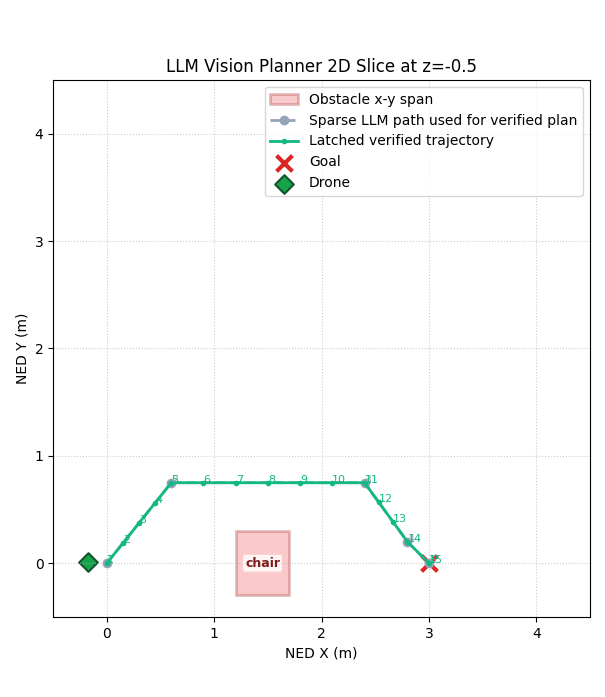
\includegraphics[width=0.86\textwidth]{Figure_1.png}
\caption{Sparse waypoint sequence generated by the LLM.}
\label{fig:sparse-waypoints}
\end{figure}



\section{Reproducibility Statement}

The implementation is reproducible on the ModalAI Starling platform using the provided repository and README instructions. Complete reproducibility may be partially limited by hardware availability, real-time onboard sensor streams, and environmental variations during physical experiments. The project intentionally prioritizes real-world deployment over simulation-only validation.

A full simulation environment was not developed because matching the exact hardware testbed specifications proved difficult, integrating the Starling platform into simulation required additional UAV model development, and the existing perception stack already operated on the real hardware. To compensate for limited hardware accessibility, the submission includes demonstration videos, trajectory plots, verification logs, execution traces, and repository instructions.

\section{Discussion}

The experiments demonstrate that LLMs can serve as effective high-level semantic planners when combined with refinement pipelines, verification layers, and robust perception systems. Rather than replacing traditional planners, LLMs complement them by introducing semantic awareness, contextual reasoning, human-aligned planning, and natural language interpretability.

Traditional planners remain superior in geometric guarantees, numerical precision, and mathematically optimal search. However, they fundamentally lack semantic understanding and human-context awareness. This work shows that combining LLM-based semantic reasoning, traditional geometric refinement, and verification-based safety filtering provides a promising direction for future UAV navigation systems.

One important lesson from the hardware implementation is that system boundaries matter. The LLM should not directly command actuators or produce a dense control policy. It should propose a sparse route, then deterministic software should refine, verify, latch, and execute the trajectory. This architecture preserves the flexibility of natural-language planning while keeping safety checks explicit and inspectable.

\section{Future Work}

Future work may explore lightweight locally deployable LLMs, multimodal VLM architectures, continual online replanning, improved verification strategies, semantic memory systems, and collaborative human-UAV interaction frameworks. Another promising direction involves distilling high-parameter cloud-based models into lightweight edge-deployable planners optimized for onboard inference.

Further research may also investigate dynamic obstacle handling, multi-agent coordination, semantic scene understanding, uncertainty-aware verification, and tighter integration between semantic labels and geometric path costs. Ultimately, this project demonstrates that LLMs possess significant potential for high-level autonomous UAV mission planning when appropriately augmented with perception, refinement, and verification tools.

\end{document}
